\chapter{偏振与部分相干}
\label{ch:05}

\section{效果}
\label{sec:ch04-effect}

读完本章，你应能：
\begin{enumerate}
  \item 说明线偏光、检偏与马吕斯定律如何改变到达相机的通量，以及这与「对比度」而非单纯「变暗」的关系；
  \item 区分完全相干、非相干与部分相干对干涉可见度 $V$ 的影响，并联系第~\ref{ch:04}~章的相干长度直觉；
  \item 解释粗糙表面在高相干照明下为何出现散斑，散斑如何抬高相位/匹配误差；
  \item 在高反牙面、金属器械、投影仪–相机光路中，设计「是否加偏振片」的利弊账（对比度 vs $\SNR$）。
\end{enumerate}

\section{原理}
\label{sec:ch04-principle}

\subsection{偏振态：够用语言}

光波电场振动方向构成偏振态。自然光可视为快速随机取向的混合；线偏光电场沿固定方向；圆偏光末端轨迹为圆。偏振片（起偏/检偏）透振方向只允许某一线偏振分量高效通过。理想线起偏后经检偏，透射强度遵循马吕斯关系
\begin{equation}
  I = I_{\mathrm{pol}}\cos^{2}\theta,
  \label{eq:ch05-malus}
\end{equation}
$\theta$ 为两透振方向夹角。$\theta=90^\circ$ 时理想消光——这是「用偏振干掉某类反射」的数学来源 \citep{HechtOptics}。

现实偏振片有限消光比、有限带宽；斜入射与镀膜还会改有效偏振态。机器视觉里常把「相机前偏振片 + 光源侧偏振」当作抑制镜面高光的一等工具，而不是装饰。

\subsection{反射：镜面保偏 vs 漫射退偏}

光滑金属或湿润釉质上的镜面反射，往往显著保留入射偏振态（方向可因入射面而旋转）；粗糙漫射或多路径次表面散射则趋向\textbf{退偏}，把光「搅」成更接近非偏振。于是：
\begin{itemize}
  \item 高光（镜面叶）与漫反射体在偏振域可分；
  \item 交叉偏振（光源线偏、相机正交检偏）常强烈压制镜面叶，留下更接近朗伯的分量；
  \item 平行偏振则可能保留高光，有时反而对标定板黑白格「加锐」，需按任务选择。
\end{itemize}

\begin{figure}[htbp]
  \centering
  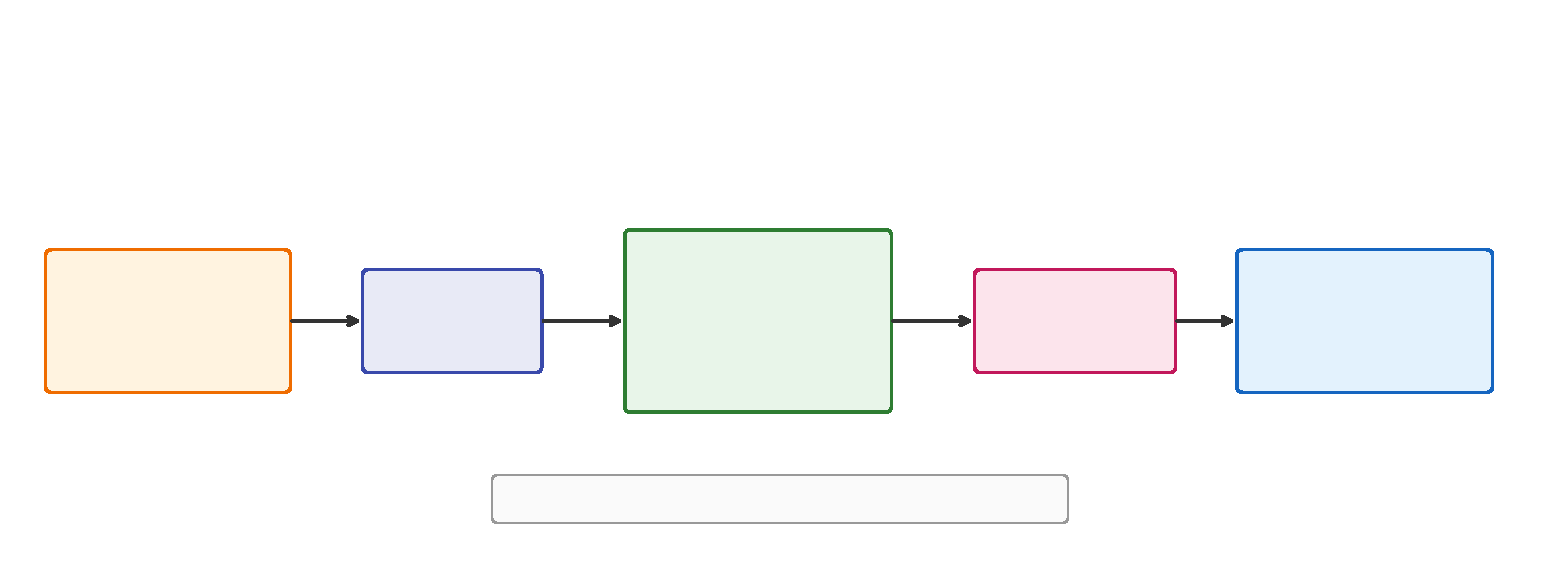
\includegraphics[width=0.95\textwidth]{fig-polarization-projector.pdf}
  \caption{投影仪–场景–相机偏振路径概念草图（非精确工程图）。镜面反射常保偏，漫射趋向退偏；检偏可抑高光，但损失通量。}
  \label{fig:ch05-polar}
\end{figure}

\subsection{部分相干与干涉可见度}
第~\ref{ch:04}~章已写 $I=I_0(1+V\cos\varphi)$。更一般地，$V$ 受振幅比与复相干度共同限制：光源在时空上完全相干时易于高 $V$；完全非相干则经典双光束干涉条纹不出现。部分相干介于二者之间：在有限光程差、有限光源角尺寸内保持可观测条纹 \citep{BornWolf,GoodmanFourierOptics}。

对结构光投影：许多系统使用 LED + 匀光 + 振幅型图案，并不依赖长程干涉；此时「部分相干」更多影响散斑多少与细微对比度。若系统本质是干涉条纹投射或外差干涉，则光源谱宽、瞳孔填充与振动稳定性直接决定 $V$。

\subsection{散斑：高相干遇到粗糙面}

相干光照射光学粗糙表面（高度起伏与 $\wavelength$ 可比）时，各面元散射的复振幅在空间随机干涉，形成颗粒状强度——散斑。散斑统计与瞳孔、波长、表面相关长度有关；对成像而言：
\begin{itemize}
  \item 散斑是乘性、空间相关的「假纹理」，会骗过立体匹配与相位估计；
  \item 增大照明孔径角、降低时间/空间相干、多波长平均、偏振分集或时间积分下的运动模糊，可抑制表观散斑对比度；
  \item 激光投影结构光必须显式管理散斑；LED 通常温和得多。
\end{itemize}

\subsection{投影仪偏振与 LCoS/DMD 直觉}

部分投影器件对偏振敏感：例如某些液晶相关架构需要特定偏振态才能高效调制；DMD（微镜）本身主要是振幅/方向开关，偏振效应来自前后偏光元件与镀膜。工程要点不是背器件手册全文，而是：
\begin{enumerate}
  \item 投影输出是否已接近线偏；
  \item 相机端再加片时，相对方位如何取（平行/正交）；
  \item 加片后通量损失多少、曝光如何补、$\SNR$ 是否掉出相位预算。
\end{enumerate}


\subsection{消光比与「假正交」}

标称交叉偏振若消光比只有 $10^{2}$--$10^{3}$，强镜面叶仍可能漏过并局部饱和。诊断时不要只看「片已正交」：看高光区是否仍顶死直方图。必要时叠中性密度、降投影局部功率，或接受该区失效掩膜。偏振片光谱透过率不平坦时，彩色三通道 $V$ 不一致，会导致依赖颜色编码的结构光出现通道间相位偏差——应用单通道或预先做通道响应校准。

\subsection{空间相干与光源角尺寸}

即使用宽谱 LED，若经小孔或细光纤再照明，空间相干性上升，粗糙面上的散斑对比度仍可能明显。扩散片、积分球匀光、增大有效光源角尺寸，是降空间相干的常用手段。代价包括：投影图案边缘变钝（又一次与 $\MTF$ 交易）、光能利用率下降。口内级小光机里，匀光与散热、体积纠缠在一起，需要在样机阶段用「静态重复扫描残差是否钉住」来验收散斑，而不是只看单帧好看。

\subsection{与辐射度的衔接}

偏振片插入后，式中的有效 $\Phi$ 与像面 $E$ 同步下降。第~\ref{ch:06}~章的 $\SNR$ 预算必须\textbf{在最终偏振配置下}重测；先在无偏振下估好再加片，会系统性乐观。反之，若交叉偏振消除了饱和，有效动态范围变宽，可能使中等灰度区的实际 $\SNR$ 改善——利弊不能只看平均 DN。

\subsection{推导：马吕斯定律从场投影来}

马吕斯定律是电场投影的平方。设入射线偏光电场振幅 $E_0$，偏振方向与检偏器透光轴夹角 $\theta$。理想检偏器只让透光轴方向的分量通过：透射场 $E_0\cos\theta$，强度正比于场振幅平方，故 $I=I_0\cos^2\theta$（式~\eqref{eq:ch05-malus}）。两点前提：入射光完全偏振；检偏器理想，正交方向透射为零。

\textbf{非理想检偏器。} 实际偏振片对正交分量也有微小透射。设透光轴方向强度透射率 $T_\parallel$，正交方向 $T_\perp$，消光比 $\mathrm{ER}=T_\parallel/T_\perp$。则
\[
  I(\theta)=I_0\bigl(T_\parallel\cos^2\theta+T_\perp\sin^2\theta\bigr).
\]
交叉放置（$\theta=90^\circ$）时剩余 $I_0T_\perp=I_0T_\parallel/\mathrm{ER}$。

\textbf{装调角误差。} 即使偏振片理想，交叉角偏离 $90^\circ$ 一个小角 $\epsilon$，剩余透射比为 $\sin^2\epsilon\approx\epsilon^2$。$\epsilon=5^\circ$ 时 $\sin^25^\circ\approx0.0076$，等效消光比只有约 $130$。两种来源同时存在时，等效消光比约为
\[
  \frac{1}{\mathrm{ER}_{\mathrm{eff}}}\approx\frac{1}{\mathrm{ER}}+\epsilon^2 .
\]
这正是「假正交」的定量含义：标称消光比上千的偏振片，装歪几度就只剩一百多。

\subsection{例：交叉偏振能把高光压到多低}

数量级示意。湿润牙面上一块镜面高光，在不加检偏时比周围漫射区亮 $I_s/I_d=50$ 倍。曝光设为让漫射区落在满阱的 $50\%$。
\begin{enumerate}
  \item \textbf{不加检偏}：高光区为满阱的 $25$ 倍，严重饱和；饱和区条纹削顶，相位不可用（第~\ref{ch:06}~章）。
  \item \textbf{加交叉检偏，$\mathrm{ER}_{\mathrm{eff}}=100$}：镜面反射基本保偏，剩余 $50I_d/100=0.5I_d$；漫射光已退偏，检偏后约剩一半，$0.5I_d$。镜面残余与漫射分量相当，高光区约为漫射区的两倍亮（满阱的 $50\%$），不再饱和；但漫射区信号也减半，需要把曝光或投影亮度加倍才能恢复原来的电子数。
  \item \textbf{$\mathrm{ER}_{\mathrm{eff}}=1000$}：剩余镜面 $0.05I_d$，只占漫射信号的十分之一，高光几乎消失。
\end{enumerate}
曝光加倍后，$\mathrm{ER}_{\mathrm{eff}}=100$ 时高光区约为满阱的 $100\%$，刚好处在饱和边缘；$\mathrm{ER}_{\mathrm{eff}}=1000$ 时约为满阱的 $55\%$，安全。由此得到一条可执行的规则：所需等效消光比 $\gtrsim I_s/I_d$ 的数倍。上例中 $\mathrm{ER}_{\mathrm{eff}}$ 至少应在几百，对应装调角误差小于约 $1.8^\circ$（$\epsilon^2<10^{-3}$）。

\subsection{散斑的数量级：颗粒多大、对比多高}

完全发展的散斑（粗糙度远大于波长、照明高度相干）强度服从负指数分布，散斑对比度 $C=\sigma_I/\langle I\rangle=1$。像面上散斑颗粒的典型尺寸由成像孔径决定，量级为
\[
  \sigma_{\mathrm{sp}}\sim\lambda\,N_{F,w},\qquad N_{F,w}=N_F(1+|m|),
\]
与衍射斑同源（数量级关系，具体系数依定义）。若一个像元内包含 $n_s$ 个独立散斑颗粒，或在曝光时间内平均了 $n_s$ 个独立散斑图样，对比度降为 $C\approx1/\sqrt{n_s}$。

例（数量级示意）：$\lambda=650\,\mathrm{nm}$、$N_F=8$、$|m|=0.4$，$\sigma_{\mathrm{sp}}\sim7\,\mu\mathrm{m}$，比 $3\,\mu\mathrm{m}$ 像元还大，单像元几乎不平均，$C$ 接近 $1$。对结构光，散斑相当于一个随位置变化、但不随时间变化的乘性因子乘在条纹上：同一像素在各相移帧中看到的散斑相同，所以它主要改变 $A$ 和 $M$ 的局部值；但散斑在一个像元内不均匀，又随条纹移动而改变加权，残余部分进入相位，形成固定的颗粒状误差。降低它的手段对应 $1/\sqrt{n_s}$ 的两个出口：增大成像孔径（颗粒变小、像元内平均更多，代价是景深）；或让散斑在曝光内变化（振动漫射片、多角度照明、多波长），代价是系统复杂度。改用低相干光源（第~\ref{ch:04}~章相干长度对照表）则从根本上削弱散斑。

\subsection{与投影器件的接口}

第~\ref{ch:07}~章会讨论 DMD 与 LCoS。从本章角度预先记住一点：LCoS 靠偏振调制灰度，投影出的光本身是线偏光，其偏振方向是\emph{固定的}；DMD 不改变偏振，出射光的偏振取决于光源和照明光路。因此，交叉偏振方案的「起偏器」对 LCoS 可能已经内置，只需在相机前加检偏并对准方位；对 DMD 则需要额外起偏，并承受约一半的光损失。

\section{限度}
\label{sec:ch04-limits}

\begin{itemize}
  \item 未引入斯托克斯矢量与缪勒矩阵的完整推演；复杂多层生物组织散射需专门模型。
  \item 「交叉偏振一定改善重建」不成立：若有用信号本身是镜面叶（极光滑金属形貌），抑镜面可能删掉信息。
  \item 散斑抑制与条纹锐度常冲突：过度空间非相干化可能糊掉高频条纹。
  \item 廉价偏振片的漏光与色偏会引入通道相关误差，彩色结构光尤需标定。
\end{itemize}

\section{对象}
\label{sec:ch04-object}

\textbf{高反牙面 / 唾液膜。} 镜面高光使相机局部饱和，条纹 $V$ 在高光区崩溃，相位出现空洞或跳变。交叉偏振常能明显降高光，使漫射分量上的条纹可读；代价是进光变少——需加长曝光或提高增益，前者怕手持运动模糊，后者抬读出噪声。实践：先定偏振方位使高光最暗，再重做曝光使非高光区灰度落在线性段中部。

\textbf{金属器械入镜。} 探针、车针等进入视场时产生强反射与次级照明，污染牙面条纹。偏振有助于压金属高光；仍需算法层做饱和检测与失效标掩膜，光学不能百分百消除。

\textbf{投影仪偏振态。} 若投影已接近线偏，相机检偏方位差 $45^\circ$ 与 $90^\circ$ 的效果完全不同：应用旋转检偏快速扫描，选「高光最小且条纹 $V$ 最大」的折中角，而不是以为「理论上正交」就结束。记录该角为工艺参数，与 $K$、$R,t$ 一并纳入设备配置。

\textbf{散斑诊断。} 激光原型机点云呈颗粒状抖动、静态场景反复扫描噪声图案几乎「钉住」——高度怀疑散斑而非随机读出噪声。对策：扩散片、摆动散射片、多帧平均、换短相干光源；换匹配窗口大小通常治标不治本。


\textbf{偏振方位工艺卡。} 将检偏转台分度，对同一高反样本记录：饱和像素比例、条纹区平均 $V$、平面重复扫描 RMS。选取饱和可控且 RMS 最小的方位写入设备配置，并与温度/清洁周期一并维护。更换偏振片批次后重做该卡。

\section*{本章收束}
偏振改的是哪一路光能进相机；部分相干与散斑改的是假纹理与可见度。高反牙面与金属是对象场上的硬例子：交叉偏振常有效，但必须重做 $\SNR$ 账。下一章把 $\Phi$、$L$、$E$ 与灰度、噪声写清楚。

\section{习题}
\label{sec:ch04-exercises}

\begin{enumerate}
  \item \textbf{（概念）} 马吕斯定律下，$\theta$ 从 $0^\circ$ 转到 $60^\circ$，理想透射强度变为原来的多少？这对 $\SNR$ 意味着什么？
  \item \textbf{（概念）} 为何「图像变暗」不等于「对比度变差」？举一个交叉偏振同时使平均灰度下降、条纹 $V$ 上升的情形。
  \item \textbf{（计算）} 设加检偏后通量变为原来的 $1/4$，光子噪声限下 $\SNR$ 大致如何变？（按 $\SNR\propto\sqrt{N_{\mathrm{ph}}}$ 粗估。）
  \item \textbf{（重建场景）} 湿润牙面高光饱和，交叉偏振后高光消失但整体噪声大、细条纹发灰。给出曝光与条纹频率的调整策略。
  \item \textbf{（重建场景）} 激光结构光静态重复性差、误差图呈固定颗粒。优先怀疑标定漂移还是散斑？如何用实验区分？
  \item \textbf{（综合）} 部分相干光源使真干涉 $V$ 下降，却可能改善散斑。这对「干涉测距」与「投影纹理立体」两种系统的选型启示有何不同？
  \item \textbf{（诊断）} 金属车针进入口内视野导致局部条纹翻转难解。除偏振外，还需要光学或流程上的哪两条措施？
  \item \textbf{（推导）} 写出非理想检偏器且存在装调角误差 $\epsilon$ 时交叉透射率的表达式，并推出 $1/\mathrm{ER}_{\mathrm{eff}}\approx1/\mathrm{ER}+\epsilon^2$ 所需的近似。
  \item \textbf{（计算）} 偏振片标称 $\mathrm{ER}=500$，交叉角误差 $2^\circ$。求 $\mathrm{ER}_{\mathrm{eff}}$。若高光比 $I_s/I_d=80$，按正文规则是否够用？
  \item \textbf{（口扫场景）} 正文高光例中，若改为先降曝光、使高光不饱和，而不加偏振片，漫射区电子数变为原来的多少？按 $\SNR\propto\sqrt{N_e}$，相位噪声变为多少倍？与交叉偏振方案比较。
  \item \textbf{（计算）} 激光投影 $\lambda=520\,\mathrm{nm}$，$N_F=4$，$|m|=0.4$，像元 $2\,\mu\mathrm{m}$。估算散斑颗粒尺寸；若用振动漫射片在每帧曝光内平均 $25$ 个独立图样，散斑对比度变为多少？
  \item \textbf{（医学重建）} 皮肤表面的镜面反射较弱、次表面散射较强。交叉偏振在这里的主要作用与牙面有何不同？（提示：次表面散射光的偏振状态。）
\end{enumerate}

\section{习题讲解}
\label{sec:ch04-solutions}

\begin{enumerate}
  \item $\cos^{2}60^\circ=1/4$，强度降为 $1/4$。若读出噪声不可忽略，$\SNR$ 往往掉得比 $2$ 倍（$\sqrt{4}$）更狠；需重估曝光。
  \item 对比度/可见度看的是调制相对均值。交叉偏振去掉饱和高光后，条纹区可能从「削顶失真」恢复为高 $V$，尽管平均 DN 更低。
  \item $N_{\mathrm{ph}}\to N_{\mathrm{ph}}/4$，$\SNR\to\SNR/2$（纯泊松）。若还有固定读出噪声，下降更明显。
  \item 适当加长曝光或提高投影亮度恢复电子数；必要时略降条纹频率以适配 $\MTF$；保持检偏方位。避免只靠数字增益。
  \item 优先散斑：误差空间图案在重复扫描中高度相似。标定漂移常表现为缓慢系统性弯曲或尺度变。区分：关激光换 LED/加扩散片看颗粒是否消；或微扰照明角度看散斑是否重排而几何标定不变。
  \item 干涉测距依赖高 $V$ 与稳定相干 → 要管谱宽与振动。投影纹理立体更怕散斑假纹理 → 可牺牲相干换平滑。同一「部分相干」旋钮，两种系统拧的方向相反。
  \item 例：遮挡/避开金属进入光路的操作规范；饱和与高梯度区失效掩膜；局部降曝光或分次扫描。偏振是手段之一，不是唯一。
  \item 设入射与透光轴夹 $90^\circ-\epsilon$：$I/I_0=T_\parallel\sin^2\epsilon+T_\perp\cos^2\epsilon$。除以 $T_\parallel$ 得 $1/\mathrm{ER}_{\mathrm{eff}}=\sin^2\epsilon+\cos^2\epsilon/\mathrm{ER}$；小角下 $\sin^2\epsilon\approx\epsilon^2$、$\cos^2\epsilon\approx1$，即得。
  \item $\epsilon=2^\circ=0.0349\,\mathrm{rad}$，$\epsilon^2\approx1.22\times10^{-3}$；$1/\mathrm{ER}_{\mathrm{eff}}\approx0.002+0.00122=0.00322$，$\mathrm{ER}_{\mathrm{eff}}\approx310$。$I_s/I_d=80$ 时剩余镜面约 $80/310\approx0.26I_d$，相对检偏后漫射 $0.5I_d$ 约一半；曝光加倍后高光区约为满阱的 $76\%$，不饱和但余量不大。按「数倍于 $I_s/I_d$」的规则属勉强够用。
  \item 高光原为满阱 $25$ 倍，要压到满阱以下，曝光须降到约 $1/25$，漫射区电子数也降到 $1/25$；$\SNR$ 降为 $1/5$，相位噪声增为约 $5$ 倍。交叉偏振方案只损失一半信号（曝光加倍可补回），明显更优。另一种做法是多曝光融合，但需要更多帧。
  \item $\sigma_{\mathrm{sp}}\sim0.52\times4\times1.4\approx2.9\,\mu\mathrm{m}$，略大于像元。平均 $25$ 个独立图样后 $C\approx1/5=0.2$。
  \item 次表面散射光多次散射后基本退偏，交叉偏振会保留它、去掉表面镜面反射。牙面上交叉偏振主要用来去高光；皮肤上它反而突出了次表面散射成分（图像看起来更「均匀、深」），会加剧条纹调制度下降和深度偏置。若目标是表面几何，平行偏振（保留表面反射）有时更有利，需要实验比较。
\end{enumerate}
